%%%%%%%%%%%%%%%%%%%%%%%%%%%%%%%%%%%%%%%%%%%%%%%%%%%%%%%%%%%%%%%%%%%%%%%%%%%%%%%%

\section{Haute disponibilité (HA)}

%%%%%%%%%%%%%%%%%%%%%%%%%%%%%%%%%%%%%%%%%%%%%%%%%%%%%%%%%%%%%%%%%%%%%%%%%%%%%%%%

\begin{frame}[fragile]{Solutions de HA}

   \begin{itemize}
      \item Il existe plusieurs solutions de HA.
      \item Certaines solutions intègrent nativement le partitionnement de données.
      \item Citus fait partie des solutions HA avec partitionnement de données
      \item L'objectif de cette formation est de permettre au client d'administrer ses bases de données avec le choix des outils qu'il a réalisé
      \item Le choix réalisé est \textbf{repmgr}
   \end{itemize}

\begin{toile}
\toileurl{https://docs.citusdata.com/en/v11.2/get\_started/what\_is\_citus.html}
\toileurl{https://repmgr.org/}
\end{toile}

\end{frame}

%%%%%%%%%%%%%%%%%%%%%%%%%%%%%%%%%%%%%%%%%%%%%%%%%%%%%%%%%%%%%%%%%%%%%%%%%%%%%%%%

\begin{frame}[fragile]{Présentation de \textbf{repmgr}}

   \begin{itemize}
      \item repmgr est une solution de gestion de:
         \begin{itemize}
            \item la réplication
            \item le switchover
            \item et le failover PostgreSQL
         \end{itemize}
      \item Elle supporte les versions PostgreSQL de 9.4 à 15
      \item Elle est portée par l'entreprise EDB
   \end{itemize}

\end{frame}

%%%%%%%%%%%%%%%%%%%%%%%%%%%%%%%%%%%%%%%%%%%%%%%%%%%%%%%%%%%%%%%%%%%%%%%%%%%%%%%%

\begin{frame}[fragile]{Caractéristiques avancées de \textbf{repmgr}}

   \begin{itemize}
      \item repmgr intègre les nouveautés introduites par PostgreSQL 9.3:
         \begin{itemize}
            \item la réplication en cascade
            \item la commutation de la ligne de temps (timeline switching)
            \item et la sauvegarde de base via la réplication
         \end{itemize}
      \item Il est disponible sous la licence GPLv3
      \item La dernière version disponible pendant la rédaction de ce document est la v5.3.3
   \end{itemize}

\end{frame}

%%%%%%%%%%%%%%%%%%%%%%%%%%%%%%%%%%%%%%%%%%%%%%%%%%%%%%%%%%%%%%%%%%%%%%%%%%%%%%%%

\begin{frame}[fragile]{Notions de cluster \textbf{repmgr}}

   \begin{itemize}
      \item Les notions suivantes sont présentes dans un cluster repmgr:
      \begin{itemize}
         \item failover: Dans le cas de l'échec d'un noeud, le standby prend le relais et devient noeud primaire
         \item switchover: Dans le cas d'une opération de maintenance, le DBA choisit de réaliser une basculer vers le noeud standby
         \item fencing: Dans le cas d'une bascule failover vers le standby, il est important que l'ancien serveur primaire ne revienne pas en ligne et cause un split-brain. L'opération de fincing consiste à isoler l'ancien noeud primaire
         \item witness server (serveur témoin): Le serveur témoin sert à mettre en place un quorum pour éviter le split brain. Il ne fait pas partie du process de réplication.
         \item En cas de coupure réseau entre les différents noeuds, ceux qui voient le serveur témoin entrent dans un process de vote pour élire un nouveau primary
      \end{itemize}
   \end{itemize}

\end{frame}

%%%%%%%%%%%%%%%%%%%%%%%%%%%%%%%%%%%%%%%%%%%%%%%%%%%%%%%%%%%%%%%%%%%%%%%%%%%%%%%%

\begin{frame}[fragile]{Eléments de la solution \textbf{repmgr}}

   \begin{itemize}
      \item Les principaux éléments de la solution repmgr sont:
      \begin{itemize}
         \item le démon repmgrd: Il surveille l'état de la replication, réalise le failover en cas de défaillance du serveur primaire et envoie des notifications d'événements
         \item la commande en ligne repmgr. Elle permet d'administrer le cluster PostgreSQL
      \end{itemize}
   \end{itemize}

\end{frame}

%%%%%%%%%%%%%%%%%%%%%%%%%%%%%%%%%%%%%%%%%%%%%%%%%%%%%%%%%%%%%%%%%%%%%%%%%%%%%%%%

\begin{frame}[fragile]{Exercice - Déploiement de \textbf{repmgr}}

   \begin{itemize}
      \item repmgr est inclus dans les dépôts Yum Repository de PostgreSQL
      \item Sur les serveurs hqpg-0x et hqpg-0x-repl, lancer les commandes suivantes:
\begin{tiny}
\begin{Verbatim}[commandchars=\\\{\}]
# dnf list | grep repmgr
...
repmgr_15.x86_64                                                  5.3.3-1.rhel8                                              pgdg15       
repmgr_15-devel.x86_64                                            5.3.3-1.rhel8                                              pgdg15       
repmgr_15-llvmjit.x86_64                                          5.3.3-1.rhel8                                              pgdg15
# dnf install repmgr_15
# dnf install rsync
\end{Verbatim}
\end{tiny}
      \item Paramétrer le noeud primaire en suivant le lien: https://repmgr.org/docs/current/quickstart-postgresql-configuration.html
      \item \textbf{Remarques}: Certaines valeurs de paramètres ont changé entre les différentes versions de PostgreSQL 9.6+
   \end{itemize}

\end{frame}

%%%%%%%%%%%%%%%%%%%%%%%%%%%%%%%%%%%%%%%%%%%%%%%%%%%%%%%%%%%%%%%%%%%%%%%%%%%%%%%%

\begin{frame}[fragile]{Exercice - Création de la base de données \textbf{repmgr}}

   \begin{itemize}
      \item Au départ, le serveur hqpg-0x est choisi comme primaire
      \item Sur le serveurs hqpg-0x, lancer les commandes suivantes:
\begin{tiny}
\begin{Verbatim}[commandchars=\\\{\}]
# su - postgres
# createuser -s repmgr
# createdb repmgr -O repmgr
[postgres@localhost ~]$ psql
psql (15.2)
Saisissez « help » pour l'aide.

postgres=# ALTER USER repmgr SET search_path TO repmgr, "$user", public;
ALTER ROLE
\end{Verbatim}
\end{tiny}
   \end{itemize}

\end{frame}

%%%%%%%%%%%%%%%%%%%%%%%%%%%%%%%%%%%%%%%%%%%%%%%%%%%%%%%%%%%%%%%%%%%%%%%%%%%%%%%%

\begin{frame}[fragile]{Exercice - Paramétrage des autorisations dans \textbf{pg\_hba.conf}}

   \begin{itemize}
      \item Vérifier que les lignes suivantes sont présentes dans \textbf{pg\_hba.conf}:
\begin{tiny}
\begin{Verbatim}[commandchars=\\\{\}]
local   replication   repmgr                              trust
host    replication   repmgr      127.0.0.1/32            trust
host    replication   repmgr      10.10.10.0/24          trust

local   repmgr        repmgr                              trust
host    repmgr        repmgr      127.0.0.1/32            trust
host    repmgr        repmgr      10.10.10.0/24          trust
\end{Verbatim}
\end{tiny}
      \item Recharger le paramétrage avec la commande suivante:
\begin{tiny}
\begin{Verbatim}[commandchars=\\\{\}]
# su - postgres
# psql
SELECT pg_reload_conf();
\end{Verbatim}
\end{tiny}
   \end{itemize}

\end{frame}

%%%%%%%%%%%%%%%%%%%%%%%%%%%%%%%%%%%%%%%%%%%%%%%%%%%%%%%%%%%%%%%%%%%%%%%%%%%%%%%%

\begin{frame}[fragile]{Exercice - Préparation du serveur standby}

   \begin{itemize}
      \item Sur le serveur standby hqpg-0x-repl, ne pas créer le base de données (pas de lancement de initdb)
      \item Elle sera créée par réplication
      \item Vérifier que le répertoire /var/lib/pgsql/15/data existe, qu'il appartient à postgres et a les droits unix: \textbf{0700}
\begin{tiny}
\begin{Verbatim}[commandchars=\\\{\}]
[root@localhost 15]# pwd
/var/lib/pgsql/15
[root@localhost 15]# ls -lrt
total 4
drwx------. 2 postgres postgres    6 10 nov.  02:29 backups
-rw-------. 1 postgres postgres 1196 29 janv. 17:51 initdb.log
\textbf{drwx------.} 2 postgres postgres    6 27 févr. 05:29 data
\end{Verbatim}
\end{tiny}
   \end{itemize}

\end{frame}

%%%%%%%%%%%%%%%%%%%%%%%%%%%%%%%%%%%%%%%%%%%%%%%%%%%%%%%%%%%%%%%%%%%%%%%%%%%%%%%%

\begin{frame}[fragile]{Exercice - Vérification du flux PostgreSQL entre le standby et le primaire}

   \begin{itemize}
      \item Vérification que le flux PostgreSQL est ouvert entre les serveurs hqpg-0x-repl et hqpg-0x
      \item Depuis le serveur hqpg-0x-repl, lancer la commande suivante en précisant l'adresse IP du serveur hqpg-0x:
\begin{tiny}
\begin{Verbatim}[commandchars=\\\{\}]
[linagora@localhost ~]$ psql 'host=10.10.10.28 user=repmgr dbname=repmgr connect_timeout=2'
psql (15.1, serveur 15.2)
Saisissez « help » pour l'aide.

repmgr=# 
\end{Verbatim}
\end{tiny}
   \end{itemize}

\end{frame}

%%%%%%%%%%%%%%%%%%%%%%%%%%%%%%%%%%%%%%%%%%%%%%%%%%%%%%%%%%%%%%%%%%%%%%%%%%%%%%%%

\begin{frame}[fragile]{Exercice - Déploiement de \textbf{repmgr.conf}}

   \begin{itemize}
      \item Sur le serveur primaire hqpg-0x, créer le fichier /etc/repmgr/15/\textbf{repmgr.conf} ci-dessous
      \item Il est important de ne pas le créer dans le répertoire data car il risque d'être écrasé ou supprimé par les opérations de réplication
\begin{tiny}
\begin{Verbatim}[commandchars=\\\{\}]
node_id=1
node_name='node1'
conninfo='host=10.10.10.28 user=repmgr dbname=repmgr connect_timeout=2'
data_directory='/var/lib/pgsql/15/data'
\end{Verbatim}
\end{tiny}
   \end{itemize}

\begin{toile}
\toileurl{https://repmgr.org/docs/current/quickstart-repmgr-conf.html}
\end{toile}

\end{frame}

%%%%%%%%%%%%%%%%%%%%%%%%%%%%%%%%%%%%%%%%%%%%%%%%%%%%%%%%%%%%%%%%%%%%%%%%%%%%%%%%

\begin{frame}[fragile]{Exercice - Enregistrement du serveur primaire}

   \begin{itemize}
      \item Pour enregistrer le serveur primaire, lancer la commande suivante:
\begin{tiny}
\begin{Verbatim}[commandchars=\\\{\}]
# su - postgres
[postgres@localhost ~]$ /usr/pgsql-15/bin/repmgr -f /etc/repmgr/15/repmgr.conf primary register                                                                                              
INFO: connecting to primary database...
NOTICE: attempting to install extension "repmgr"
NOTICE: "repmgr" extension successfully installed
NOTICE: primary node record (ID: 1) registered
\end{Verbatim}
\end{tiny}
      \item Vérifier le résultat de la commande:
\begin{tiny}
\begin{Verbatim}[commandchars=\\\{\}]
[postgres@localhost ~]$ /usr/pgsql-15/bin/repmgr -f /etc/repmgr/15/repmgr.conf cluster show
 ID | Name  | Role    | Status    | Upstream | Location | Priority | Timeline | Connection string                                           
----+-------+---------+-----------+----------+----------+----------+----------+--------------------------------------------------------------
 1  | node1 | primary | * running |          | default  | 100      | 2        | host=10.10.10.28 user=repmgr dbname=repmgr connect_timeout=2
\end{Verbatim}
\end{tiny}
   \end{itemize}

\begin{toile}
\toileurl{https://repmgr.org/docs/current/quickstart-primary-register.html}
\end{toile}

\end{frame}

%%%%%%%%%%%%%%%%%%%%%%%%%%%%%%%%%%%%%%%%%%%%%%%%%%%%%%%%%%%%%%%%%%%%%%%%%%%%%%%%

\begin{frame}[fragile]{Exercice - Vérification en base}

   \begin{itemize}
      \item Vérification en base
\begin{tiny}
\begin{Verbatim}[commandchars=\&\{\}]
[postgres@localhost ~]$ psql repmgr
psql (15.2)
Saisissez « help » pour l'aide.

repmgr=# \x
Affichage étendu activé.
repmgr=# select * from repmgr.nodes;
-[ RECORD 1 ]----+-------------------------------------------------------------
node_id          | 1
upstream_node_id | 
active           | t
node_name        | node1
type             | primary
location         | default
priority         | 100
conninfo         | host=10.10.10.28 user=repmgr dbname=repmgr connect_timeout=2
repluser         | repmgr
slot_name        | 
config_file      | /etc/repmgr/15/repmgr.conf
\end{Verbatim}
\end{tiny}
   \end{itemize}

\begin{toile}
\toileurl{https://repmgr.org/docs/current/quickstart-primary-register.html}
\end{toile}

\end{frame}

%%%%%%%%%%%%%%%%%%%%%%%%%%%%%%%%%%%%%%%%%%%%%%%%%%%%%%%%%%%%%%%%%%%%%%%%%%%%%%%%

\begin{frame}[fragile]{Exercice - Clone du primaire vers le standby}

   \begin{itemize}
      \item Sur le serveur standby hqpg-0x-repl, créer le fichier /etc/repmgr/15/\textbf{repmgr.conf} ci-dessous
      \item Il est important de ne pas le créer dans le répertoire data car il risque d'être écrasé ou supprimé par les opérations de réplication
\begin{tiny}
\begin{Verbatim}[commandchars=\\\{\}]
node_id=2
node_name='node2'
conninfo='host=10.10.10.29 user=repmgr dbname=repmgr connect_timeout=2'
data_directory='/var/lib/pgsql/15/data'
\end{Verbatim}
\end{tiny}
   \end{itemize}

\begin{toile}
\toileurl{https://repmgr.org/docs/current/quickstart-standby-clone.html}
\end{toile}

\end{frame}

%%%%%%%%%%%%%%%%%%%%%%%%%%%%%%%%%%%%%%%%%%%%%%%%%%%%%%%%%%%%%%%%%%%%%%%%%%%%%%%%

\begin{frame}[fragile]{Exercice - Clone du primaire vers le standby en mode dry-run}

   \begin{itemize}
      \item Sur le serveur standby, lancer la commande suivante avec le user postgres:
\begin{tiny}
\begin{Verbatim}[commandchars=\&\{\}]
$ /usr/pgsql-15/bin/repmgr -h 10.10.10.28 -U repmgr -d repmgr \
-f /etc/repmgr/15/repmgr.conf standby clone --dry-run
NOTICE: destination directory "/var/lib/pgsql/15/data" provided
INFO: connecting to source node
DETAIL: connection string is: host=10.10.10.28 user=repmgr dbname=repmgr
DETAIL: current installation size is 51 MB
INFO: "repmgr" extension is installed in database "repmgr"
INFO: replication slot usage not requested;  no replication slot will be set up for this standby
INFO: parameter "max_wal_senders" set to 10
NOTICE: checking for available walsenders on the source node (2 required)
INFO: sufficient walsenders available on the source node
DETAIL: 2 required, 10 available
NOTICE: checking replication connections can be made to the source server (2 required)
INFO: required number of replication connections could be made to the source server
DETAIL: 2 replication connections required
WARNING: data checksums are not enabled and "wal_log_hints" is "off"
DETAIL: pg_rewind requires "wal_log_hints" to be enabled
NOTICE: standby will attach to upstream node 1
HINT: consider using the -c/--fast-checkpoint option
INFO: would execute:
  pg_basebackup -l "repmgr base backup"  -D /var/lib/pgsql/15/data -h 10.10.10.28 -p 5432 -U repmgr -X stream 
INFO: all prerequisites for "standby clone" are met
\end{Verbatim}
\end{tiny}
      \item Activer \textbf{wal\_log\_hints} pour corriger le WARNING
   \end{itemize}

\end{frame}

%%%%%%%%%%%%%%%%%%%%%%%%%%%%%%%%%%%%%%%%%%%%%%%%%%%%%%%%%%%%%%%%%%%%%%%%%%%%%%%%

\begin{frame}[fragile]{Exercice - Clone du primaire vers le standby en mode production}

   \begin{itemize}
      \item Relancer la commande précédente sans l'option --dry-run si aucun erreur ou warning n'est indiqué
\begin{tiny}
\begin{Verbatim}[commandchars=\&\{\}]
$ /usr/pgsql-15/bin/repmgr -h 10.10.10.28 -U repmgr -d repmgr \
-f /etc/repmgr/15/repmgr.conf standby clone
NOTICE: destination directory "/var/lib/pgsql/15/data" provided
INFO: connecting to source node
DETAIL: connection string is: host=10.10.10.28 user=repmgr dbname=repmgr
DETAIL: current installation size is 51 MB
INFO: replication slot usage not requested;  no replication slot will be set up for this standby                                                                                             
NOTICE: checking for available walsenders on the source node (2 required)
NOTICE: checking replication connections can be made to the source server (2 required)
INFO: checking and correcting permissions on existing directory "/var/lib/pgsql/15/data"
NOTICE: starting backup (using pg_basebackup)...
HINT: this may take some time; consider using the -c/--fast-checkpoint option
INFO: executing:
  pg_basebackup -l "repmgr base backup"  -D /var/lib/pgsql/15/data -h 10.10.10.28 -p 5432 -U repmgr -X stream                                                                                
NOTICE: standby clone (using pg_basebackup) complete
NOTICE: you can now start your PostgreSQL server
HINT: for example: pg_ctl -D /var/lib/pgsql/15/data start
HINT: after starting the server, you need to register this standby with "repmgr standby register"
\end{Verbatim}
\end{tiny}
   \end{itemize}

\end{frame}

%%%%%%%%%%%%%%%%%%%%%%%%%%%%%%%%%%%%%%%%%%%%%%%%%%%%%%%%%%%%%%%%%%%%%%%%%%%%%%%%

\begin{frame}[fragile]{Exercice - Démarrage du serveur standby}

   \begin{itemize}
      \item Démarrer le serveur standby avec la commande suivante:
\begin{tiny}
\begin{Verbatim}[commandchars=\&\{\}]
$ /usr/pgsql-15/bin/pg_ctl -D /var/lib/pgsql/15/data start
\end{Verbatim}
\end{tiny}
   \end{itemize}

\end{frame}

%%%%%%%%%%%%%%%%%%%%%%%%%%%%%%%%%%%%%%%%%%%%%%%%%%%%%%%%%%%%%%%%%%%%%%%%%%%%%%%%

\begin{frame}[fragile]{Exercice - Vérification de la réplication depuis le noeud primaire}

   \begin{itemize}
      \item Sur le serveur primaire hqpg-0x, lancer la commande suivante:
\begin{tiny}
\begin{Verbatim}[commandchars=\&\{\}]
postgres=# SELECT * FROM pg_stat_replication;
-[ RECORD 1 ]----+------------------------------
pid              | 88219
usesysid         | 43973
usename          | repmgr
application_name | node2
client_addr      | 10.10.10.29
client_hostname  | 
client_port      | 34828
backend_start    | 2023-02-27 07:52:15.110657-05
backend_xmin     | 
state            | streaming
sent_lsn         | 0/3117D458
write_lsn        | 0/3117D458
flush_lsn        | 0/3117D458
replay_lsn       | 0/310001C8
write_lag        | 00:00:00.038475
flush_lag        | 00:00:00.113213
replay_lag       | 00:05:19.386491
sync_priority    | 0
sync_state       | async
reply_time       | 2023-02-27 07:57:34.59643-05

\end{Verbatim}
\end{tiny}
   \end{itemize}

\end{frame}

%%%%%%%%%%%%%%%%%%%%%%%%%%%%%%%%%%%%%%%%%%%%%%%%%%%%%%%%%%%%%%%%%%%%%%%%%%%%%%%%

\begin{frame}[fragile]{Exercice - Vérification de la réplication depuis le noeud standby}

   \begin{itemize}
      \item Sur le serveur standby hqpg-0x-repl, lancer la commande suivante:
\begin{tiny}
\begin{Verbatim}[commandchars=\&\{\}]
postgres=# SELECT * FROM pg_stat_wal_receiver;
-[ RECORD 1 ]---------+-----------------------------------------------------------------------------------------------------------------------------------------------------------------------------------------------------------------------------------------------------------------------------------------------------------------------------------------                           
pid                   | 42326
status                | streaming
receive_start_lsn     | 0/31000000
receive_start_tli     | 2
written_lsn           | 0/3117D578
flushed_lsn           | 0/3117D578
received_tli          | 2
last_msg_send_time    | 2023-02-27 08:01:37.164908-05
last_msg_receipt_time | 2023-02-27 08:01:37.165114-05
latest_end_lsn        | 0/3117D578
latest_end_time       | 2023-02-27 07:59:06.918943-05
slot_name             |
sender_host           | 10.10.10.28
sender_port           | 5432
conninfo              | user=repmgr passfile=/var/lib/pgsql/.pgpass channel_binding=prefer connect_timeout=2 dbname=replication host=10.10.10.28 port=5432 application_name=node2 fallback_application_name=walreceiver sslmode=prefer sslcompression=0 sslsni=1 ssl_min_protocol_version=TLSv1.2 gssencmode=prefer krbsrvname=postgres target_session_attrs=any                           
\end{Verbatim}
\end{tiny}
   \end{itemize}

\end{frame}

%%%%%%%%%%%%%%%%%%%%%%%%%%%%%%%%%%%%%%%%%%%%%%%%%%%%%%%%%%%%%%%%%%%%%%%%%%%%%%%%

\begin{frame}[fragile]{Exercice - Enregistrement du noeud standby}

   \begin{itemize}
      \item Sur le serveur standby hqpg-0x-repl, lancer la commande suivante avec le user postgres:
\begin{tiny}
\begin{Verbatim}[commandchars=\&\{\}]
$ /usr/pgsql-15/bin/repmgr -f /etc/repmgr/15/repmgr.conf standby register
INFO: connecting to local node "node2" (ID: 2)
INFO: connecting to primary database
WARNING: --upstream-node-id not supplied, assuming upstream node is primary (node ID: 1)
INFO: standby registration complete
NOTICE: standby node "node2" (ID: 2) successfully registered
\end{Verbatim}
\end{tiny}
      \item Sur le serveur primaire hqpg-0x, vérifier l'état du cluster avec la commande suivante:
\begin{tiny}
\begin{Verbatim}[commandchars=\&\{\}]
[postgres@localhost pg_wal]$ /usr/pgsql-15/bin/repmgr -f /etc/repmgr/15/repmgr.conf cluster show
 ID | Name  | Role    | Status    | Upstream | Location | Priority | Timeline | Connection string                                           
----+-------+---------+-----------+----------+----------+----------+----------+--------------------------------------------------------------
 1  | node1 | primary | * running |          | default  | 100      | 2        | host=10.10.10.28 user=repmgr dbname=repmgr connect_timeout=2
 2  | node2 | standby |   running | ? node1  | default  | 100      | 2        | host=10.10.10.29 user=repmgr dbname=repmgr connect_timeout=2

WARNING: following issues were detected
  - WAL replay is paused on node "node2" (ID: 2) with WAL replay pending; this node cannot be manually promoted until WAL replay is resumed
\end{Verbatim}
\end{tiny}
   \end{itemize}

\end{frame}

%%%%%%%%%%%%%%%%%%%%%%%%%%%%%%%%%%%%%%%%%%%%%%%%%%%%%%%%%%%%%%%%%%%%%%%%%%%%%%%%

\begin{frame}[fragile]{Exercice - Réactivation du rejeu des WALs}

   \begin{itemize}
      \item Réactivation du rejeu des WALs
\begin{tiny}
\begin{Verbatim}[commandchars=\&\{\}]
repmgr=# select pg_wal_replay_resume()
;
 pg_wal_replay_resume
----------------------

(1 ligne)


[postgres@localhost pg_wal]$ /usr/pgsql-15/bin/repmgr -f /etc/repmgr/15/repmgr.conf cluster show                                                                                             
 ID | Name  | Role    | Status               | Upstream | Location | Priority | Timeline | Connection string                                                                                 
----+-------+---------+----------------------+----------+----------+----------+----------+--------------------------------------------------------------                                     
 1  | node1 | primary | * running            |          | default  | 100      | 2        | host=10.10.10.28 user=repmgr dbname=repmgr connect_timeout=2                                      
 2  | node2 | standby | ! running as primary | ? node1  | default  | 100      | 3        | host=10.10.10.29 user=repmgr dbname=repmgr connect_timeout=2                                      

WARNING: following issues were detected
  - node "node2" (ID: 2) is registered as standby but running as primary
\end{Verbatim}
\end{tiny}
   \end{itemize}

\end{frame}

%%%%%%%%%%%%%%%%%%%%%%%%%%%%%%%%%%%%%%%%%%%%%%%%%%%%%%%%%%%%%%%%%%%%%%%%%%%%%%%%

\begin{frame}[fragile]{Exercice - Test du failover avec \textbf{repmgrd}}

   \begin{itemize}
      \item Sur le serveur hqpg-0x-repl, lancer le process \textbf{repmgrd}
\begin{tiny}
\begin{Verbatim}[commandchars=\&\{\}]
$ /usr/pgsql-15/bin/repmgrd -f /etc/repmgr/15/repmgr.conf
\end{Verbatim}
\end{tiny}
      \item Celui-ci se met en surveillance du noeud principal et détecte les cas d'indisponibilité
      \item Arrêter le noeud primaire avec la commande ci-dessous lancée en tant que root:
\begin{tiny}
\begin{Verbatim}[commandchars=\&\{\}]
# systemctl stop postgresql-15.service
\end{Verbatim}
      \item Vérifier que le noeud réplicat devient noeud primaire
\end{tiny}
   \end{itemize}

\end{frame}

%%%%%%%%%%%%%%%%%%%%%%%%%%%%%%%%%%%%%%%%%%%%%%%%%%%%%%%%%%%%%%%%%%%%%%%%%%%%%%%%

\begin{frame}[fragile]{Exercice - Rattrapage de l'ancien primaire vers le nouveau primaire}

   \begin{itemize}
      \item Le lien suivant décrit comment le nouveau réplicat (ancien primaire) rattrape le nouveau primaire
      \item https://repmgr.org/docs/current/follow-new-primary.html
   \end{itemize}

\end{frame}

%%%%%%%%%%%%%%%%%%%%%%%%%%%%%%%%%%%%%%%%%%%%%%%%%%%%%%%%%%%%%%%%%%%%%%%%%%%%%%%%

\section{Partitionnement des données}

%%%%%%%%%%%%%%%%%%%%%%%%%%%%%%%%%%%%%%%%%%%%%%%%%%%%%%%%%%%%%%%%%%%%%%%%%%%%%%%%

\begin{frame}[fragile]{Présentation des indexes B-Tree}

   \begin{itemize}
      \item Un index de type B-Tree est un arbre composé:
      \begin{itemize}
         \item d'une racine
         \item de noeuds intermédiaires
         \item de feuilles
      \end{itemize}
      \item Les feuilles correspondent aux données dans les tables
      \item Chaque noeud intermédiaire porte un nombre de \textbf{clefs} maximum et minimum

   \end{itemize}

\begin{toile}
\toileurl{https://en.wikipedia.org/wiki/B-tree}
\toileurl{https://www.postgresql.org/docs/15/btree.html}
\toileurl{https://www.postgresql.org/docs/15/btree-implementation.html}
\end{toile}

\end{frame}

%%%%%%%%%%%%%%%%%%%%%%%%%%%%%%%%%%%%%%%%%%%%%%%%%%%%%%%%%%%%%%%%%%%%%%%%%%%%%%%%

\begin{frame}[fragile]{Présentation des indexes B-Tree}

   \begin{itemize}
      \item Les \textbf{clés} définissent les bornes minimum et maximum des valeurs portées par les noeuds enfants
      \item Lorsqu'un noeud atteint son nombre maximum d'enfants, une scission ("split") a lieu
      \item Lorsqu'un noeud atteint son nombre minimum d'enfants, une fusion ("merge") a lieu

   \end{itemize}

\end{frame}

%%%%%%%%%%%%%%%%%%%%%%%%%%%%%%%%%%%%%%%%%%%%%%%%%%%%%%%%%%%%%%%%%%%%%%%%%%%%%%%%

\begin{frame}[fragile]{L'objectif des indexes B-Tree}

   \begin{itemize}
      \item L'objectif de l'index B-Tree est de stocker en mémoire une partie d'un index très volumineux
      \item Cet objectif est atteint par le fait que les noeuds intermédiaires indexent des plages de données
   \end{itemize}

\end{frame}

%%%%%%%%%%%%%%%%%%%%%%%%%%%%%%%%%%%%%%%%%%%%%%%%%%%%%%%%%%%%%%%%%%%%%%%%%%%%%%%%

\begin{frame}[fragile]{Schéma explicatif des indexes B-Tree}

\begin{figure}
\begin{center}
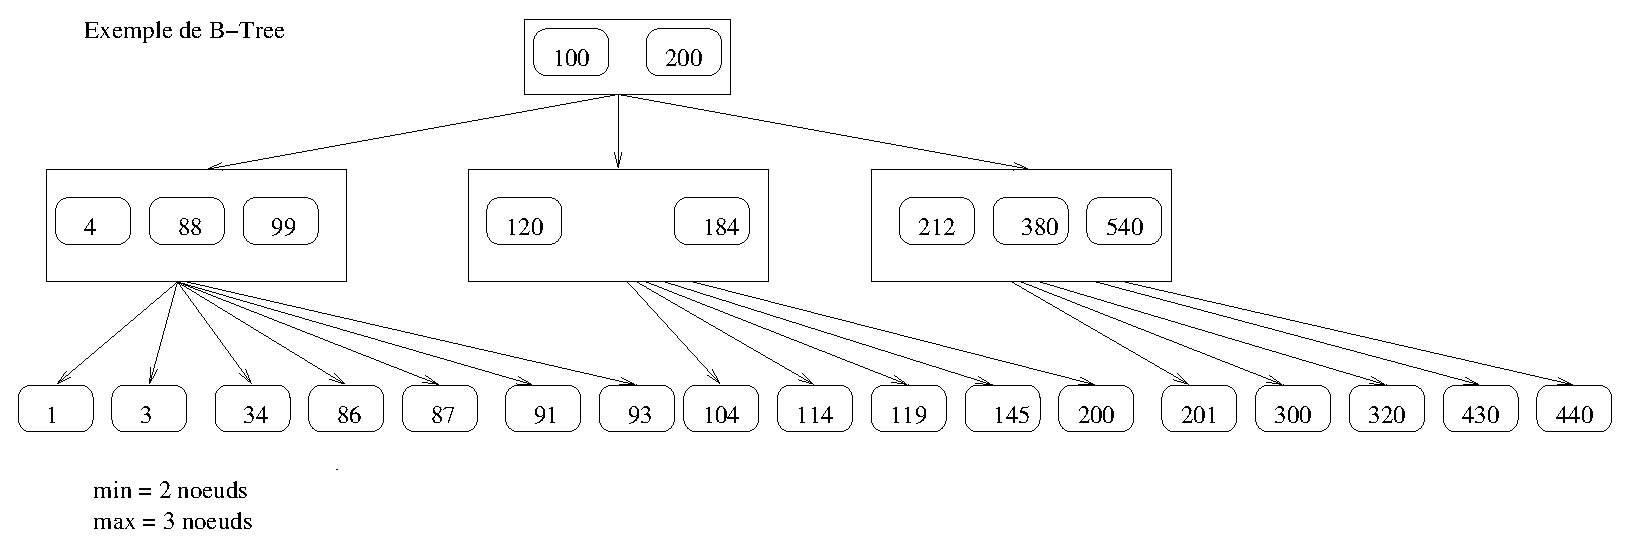
\includegraphics[angle=0, width=0.5\textwidth]{images/b_tree.eps}
\end{center}
\end{figure}

\end{frame}

%%%%%%%%%%%%%%%%%%%%%%%%%%%%%%%%%%%%%%%%%%%%%%%%%%%%%%%%%%%%%%%%%%%%%%%%%%%%%%%%

\begin{frame}[fragile]{Tables partitionnées}

   \begin{itemize}
      \item PostgreSQL supporte le partitionnement de données.
      \item Le partitionnement PostgreSQL consiste à découper une table logique en plusieurs petits morceaux physiques

   \end{itemize}

\begin{toile}
\toileurl{https://www.postgresql.org/docs/15/ddl-partitioning.html}
\end{toile}

\end{frame}

%%%%%%%%%%%%%%%%%%%%%%%%%%%%%%%%%%%%%%%%%%%%%%%%%%%%%%%%%%%%%%%%%%%%%%%%%%%%%%%%

\begin{frame}[fragile]{Tables partitionnées}

   \begin{itemize}
      \item Dans certaines situations, le partitionnement a plusieurs avantages:
      \begin{itemize}
         \item lorsque les données accédées sont localisées dans une partition ou un nombre réduit de partitions. A ce moment, la partie haute des indexes (B-Tree) qui correspond à ces données est entièrement en cache.
         \item lorsque les données modifiées ou accédée couvrent la majorité de la partition, il est préférable d'utiliser un scan séquentiel au lieu d'utiliser un index
         \item les chargements de données massifs ou suppressions massives de données correspondant à une partition sont réalisés en ajoutant une partition ou en supprimant une partition. En cas de suppression massive, un \textbf{VACUUM} est économisé
         \item les données ou partitions les moins utilisées peuvent être migrées vers des disques moins onéreux et moins rapides
      \end{itemize}

   \end{itemize}

\end{frame}

%%%%%%%%%%%%%%%%%%%%%%%%%%%%%%%%%%%%%%%%%%%%%%%%%%%%%%%%%%%%%%%%%%%%%%%%%%%%%%%%

\begin{frame}[fragile]{A quel moment faire le choix d'une table partitionnée}

   \begin{itemize}
      \item Il peut être intéressant de partitionner une table lorsque sa taille dépasse celle de la quantité de RAM du serveur
      \item Il existe différents types de partitionnement:
      \begin{itemize}
         \item Partitionnement par plage (Range partitioning)
         \item Partitionnement par liste (List partitioning)
         \item Partitionnement par hash (Hash partitioning)
      \end{itemize}

   \end{itemize}

\end{frame}

%%%%%%%%%%%%%%%%%%%%%%%%%%%%%%%%%%%%%%%%%%%%%%%%%%%%%%%%%%%%%%%%%%%%%%%%%%%%%%%%

\begin{frame}[fragile]{Partitionnement par plage (Range partitioning)}

   \begin{itemize}
      \item La plage de valeurs est portée par une ou plusieurs colonnes
      \item Les valeurs peuvent être de type date ou identifiants
      \item Les plages n'ont pas d'intersection: elles n'ont pas de valeurs en commun
      \item Le min de la plage est inclus, le max est exclus
   \end{itemize}

\end{frame}

%%%%%%%%%%%%%%%%%%%%%%%%%%%%%%%%%%%%%%%%%%%%%%%%%%%%%%%%%%%%%%%%%%%%%%%%%%%%%%%%

\begin{frame}[fragile]{Partitionnement par liste (List partitioning)}

   \begin{itemize}
      \item La plage de valeurs est définie par une liste qui indique les valeurs autorisées dans la partition
   \end{itemize}

\end{frame}

%%%%%%%%%%%%%%%%%%%%%%%%%%%%%%%%%%%%%%%%%%%%%%%%%%%%%%%%%%%%%%%%%%%%%%%%%%%%%%%%

\begin{frame}[fragile]{Partitionnement par hash (Hash partitioning)}

   \begin{itemize}
      \item La clé de partitionnement est définie par un modulo et un reste
      \item La valeur est autorisée dans la partition lorsque son modulo est égale au reste de la partition
   \end{itemize}

\end{frame}

%%%%%%%%%%%%%%%%%%%%%%%%%%%%%%%%%%%%%%%%%%%%%%%%%%%%%%%%%%%%%%%%%%%%%%%%%%%%%%%%

\begin{frame}[fragile]{Stockage des tables partitionnées}

   \begin{itemize}
      \item Une table partitionnée est virtuelle. Elle ne possède pas de stockage.
      \item Ce sont ses partitions qui occupent du stockage
      \item Chaque partitiotn récupère une partie des données de la table
      \item Chaque ligne est oritentée vers la partition en fonction de la valeur de la clef de partition
      \item Lorsque la clef de partition est mise à jour, la ligne est déplacée vers la parition qui correspond à la nouvelle clef
   \end{itemize}

\end{frame}

%%%%%%%%%%%%%%%%%%%%%%%%%%%%%%%%%%%%%%%%%%%%%%%%%%%%%%%%%%%%%%%%%%%%%%%%%%%%%%%%

\begin{frame}[fragile]{Sous partitions}

   \begin{itemize}
      \item Une partition peut elle même être partitionnée
      \item Les partitions ont les mêmes colonnes que leurs parents
      \item Cependant, elles peuvent définir leurs propres indexes, valeurs par défaut et contraintes
   \end{itemize}

\begin{toile}
\toileurl{https://www.postgresql.org/docs/15/sql-createtable.html}
\end{toile}

\end{frame}

%%%%%%%%%%%%%%%%%%%%%%%%%%%%%%%%%%%%%%%%%%%%%%%%%%%%%%%%%%%%%%%%%%%%%%%%%%%%%%%%

\begin{frame}[fragile]{Conversion des tables en tables partitionnées}

   \begin{itemize}
      \item Il n'est pas possible de transformer une table en une table partitionnée et inversement
      \item Il est possible d'ajouter une partition à une table partionnée
      \item Il est possible d'ajouter une table partitionnée à une table partionnée en tant que partition
      \item Il est possible de transformer une partition d'une table en une table régulière
      \item Ces possibilités facilitent la maintenance des tables partitionnées
      \item Les tables étrangères (\textbf{foreign tables}) peuvent jouer aussi le rôle de partitions
   \end{itemize}

\begin{toile}
\toileurl{https://www.postgresql.org/docs/15/sql-altertable.html}
\toileurl{https://www.postgresql.org/docs/15/ddl-foreign-data.html}
\end{toile}

\end{frame}

%%%%%%%%%%%%%%%%%%%%%%%%%%%%%%%%%%%%%%%%%%%%%%%%%%%%%%%%%%%%%%%%%%%%%%%%%%%%%%%%

\begin{frame}[fragile]{\textbf{enable\_partition\_pruning}}

   \begin{itemize}
      \item Ce paramètre autorise le planificateur de requêtes d'élaguer certaines partitions de tables de son plan d'exécution
      \item Valeur par défaut \textbf{on}
   \end{itemize}

\begin{toile}
\toileurl{https://www.postgresql.org/docs/15/runtime-config-query.html\#GUC-ENABLE-PARTITION-PRUNING}
\end{toile}

\end{frame}

%%%%%%%%%%%%%%%%%%%%%%%%%%%%%%%%%%%%%%%%%%%%%%%%%%%%%%%%%%%%%%%%%%%%%%%%%%%%%%%%

\begin{frame}[fragile]{Exercice - Manipuler des tables partitionnées}

   \begin{itemize}
      \item Suivre l'exercice paragraphe Example dans https://www.postgresql.org/docs/15/ddl-partitioning.html
      \item Créer une table partitionnée
      \item Ajouter une sous-partition
      \item Ajouter un index à une partition
   \end{itemize}

\end{frame}

%%%%%%%%%%%%%%%%%%%%%%%%%%%%%%%%%%%%%%%%%%%%%%%%%%%%%%%%%%%%%%%%%%%%%%%%%%%%%%%%

\begin{frame}[fragile]{Maintenance des partitions - Suppression d'une partition}

   \begin{itemize}
      \item Il y a 2 possibilités pour supprimer une partition d'une table:
\begin{tiny}
\begin{Verbatim}[commandchars=\\\{\}]
   DROP TABLE measurement\_y2006m02;
\end{Verbatim}
\end{tiny}
      \item L'autre possibilité est:
\begin{tiny}
\begin{Verbatim}[commandchars=\\\{\}]
ALTER TABLE measurement DETACH PARTITION measurement\_y2006m02;
-- ou
ALTER TABLE measurement DETACH PARTITION measurement\_y2006m02 \textbf{CONCURRENTLY};
\end{Verbatim}
\end{tiny}
      \item Elle permet de réaliser un dump ou une sauvegarde de la partition avant suppression définitive
      \item La clause \textbf{CONCURRENTLY} permet une modification de la table parente en parallèle
   \end{itemize}

\end{frame}

%%%%%%%%%%%%%%%%%%%%%%%%%%%%%%%%%%%%%%%%%%%%%%%%%%%%%%%%%%%%%%%%%%%%%%%%%%%%%%%%

\begin{frame}[fragile]{Maintenance des partitions - Ajout d'une partition - \textbf{ATTACH}}

   \begin{itemize}
      \item Comme pour la suppression, il y a 2 possibilités pour ajouter une partition à une table:
\begin{tiny}
\begin{Verbatim}[commandchars=\\\{\}]
CREATE TABLE measurement_y2008m02 PARTITION OF measurement
FOR VALUES FROM ('2008-02-01') TO ('2008-03-01')
TABLESPACE fasttablespace;
\end{Verbatim}
\end{tiny}
      \item L'autre possibilité est de créer une table en dehors de la table partitionnée puis de la rattacher:
\begin{tiny}
\begin{Verbatim}[commandchars=\#\{\}]
CREATE TABLE measurement\_y2008m02
(LIKE measurement INCLUDING DEFAULTS INCLUDING CONSTRAINTS)
TABLESPACE fasttablespace;

ALTER TABLE measurement_y2008m02 ADD CONSTRAINT y2008m02
   CHECK ( logdate >= DATE '2008-02-01' AND logdate < DATE '2008-03-01' );

\copy measurement_y2008m02 from 'measurement_y2008m02'
-- possibly some other data preparation work

ALTER TABLE measurement ATTACH PARTITION measurement_y2008m02
    FOR VALUES FROM ('2008-02-01') TO ('2008-03-01' );
\end{Verbatim}
\end{tiny}
      \item Noter l'utilisation du \textbf{LIKE} qui permet de dupliquer la définition de la table
      \item \textbf{Remarque}: Il est important d'ajouter la vérification \textbf{CHECK} avant d'attacher la partition. Cela évite un scan verrouillé en \textbf{ACCESS LOCK} sur la partition.
   \end{itemize}

\end{frame}

%%%%%%%%%%%%%%%%%%%%%%%%%%%%%%%%%%%%%%%%%%%%%%%%%%%%%%%%%%%%%%%%%%%%%%%%%%%%%%%%

\begin{frame}[fragile]{Maintenance des partitions - Ajout d'une partition - \textbf{ATTACH}}

   \begin{itemize}
      \item La clause de vérification avant l'\textbf{ATTACH} est importante en cas de présence d'une partition \textbf{DEFAULT}
      \item Sans la clause \textbf{CHECK}, la partition qui est rattachée va être scannée en étant verrouillé afin de vérifier qu'il n'y a pas d'enregistrement susceptible d'aller en \textbf{DEFAULT}
   \end{itemize}

\end{frame}

%%%%%%%%%%%%%%%%%%%%%%%%%%%%%%%%%%%%%%%%%%%%%%%%%%%%%%%%%%%%%%%%%%%%%%%%%%%%%%%%

\begin{frame}[fragile]{Indexes et tables partitionnées}

   \begin{itemize}
      \item Comme vu précédemment, il est possible de créer des indexes sur des tables partitionnées
      \item Ces indexes seront appliqués aux futures partitions
      \item Il y a cependant une limitation: il n'est pas possible d'utiliser \textbf{CONCURRENTLY}. Il y a donc un verrou exclusif à l'ajout d'une partition
      \item Pour éviter cela, on utilise \textbf{CREATE INDEX ON ONLY} sur la table partitionnée
      \item L'index créé de cette manière est invalide
      \item Il est ensuite possible d'appliquer la clause \textbf{CONCURRENTLY} sur les partitions qui seront rattachées
      \item Une fois l'ensemble des partitions attachées avec l'index, celui-ci est validé
      \item Cette technique s'applique aussi aux clauses \textbf{UNIQUE} et \textbf{PRIMARY KEY}

   \end{itemize}

\end{frame}

%%%%%%%%%%%%%%%%%%%%%%%%%%%%%%%%%%%%%%%%%%%%%%%%%%%%%%%%%%%%%%%%%%%%%%%%%%%%%%%%

\begin{frame}[fragile]{Exercice - Utiliser la clause \textbf{CREATE INDEX ON ONLY}}

   \begin{itemize}
      \item Merci de réaliser l'exercice de création d'index comme indiqué dans le lien https://www.postgresql.org/docs/15/ddl-partitioning.html\#DDL-PARTITION-PRUNING
      \item au paragraphe 5.11.2.2 en utilisant CREATE INDEX ON ONLY
   \end{itemize}

\end{frame}

%%%%%%%%%%%%%%%%%%%%%%%%%%%%%%%%%%%%%%%%%%%%%%%%%%%%%%%%%%%%%%%%%%%%%%%%%%%%%%%%

\begin{frame}[fragile]{Elagage (pruning) de partitions dans le planificateur de requêtes}

   \begin{itemize}
      \item Comme vu précédemment l'élagage de partitions est activé par défaut pour le planificateur de requêtes
\begin{tiny}
\begin{Verbatim}[commandchars=\\\{\}]
SET enable_partition_pruning = on;                 -- the default
SELECT count(*) FROM measurement WHERE logdate >= DATE '2008-01-01';
\end{Verbatim}
\end{tiny}
      \item Sans l'élagage de partitions, la requête précédente aurait scanné toute la table measurement
      \item Avec l'élagage, le planificateur détermine pour chaque partition que la donnée ne s'y trouve et ne scanne pas la partition
   \end{itemize}

\end{frame}

%%%%%%%%%%%%%%%%%%%%%%%%%%%%%%%%%%%%%%%%%%%%%%%%%%%%%%%%%%%%%%%%%%%%%%%%%%%%%%%%

\begin{frame}[fragile]{Vérification avec l'EXPLAIN plan}

\begin{tiny}
\begin{Verbatim}[commandchars=\#\{\}]
SET enable_partition_pruning = \textbf{off};
EXPLAIN SELECT count(*) FROM measurement WHERE logdate >= DATE '2008-01-01';
                                    QUERY PLAN
-----------------------------------------------------------------------------------
 Aggregate  (cost=188.76..188.77 rows=1 width=8)
   ->  Append  (cost=0.00..181.05 rows=3085 width=0)
         ->  Seq Scan on measurement_y2006m02  (cost=0.00..33.12 rows=617 width=0)
               Filter: (logdate >= '2008-01-01'::date)
         ->  Seq Scan on measurement_y2006m03  (cost=0.00..33.12 rows=617 width=0)
               Filter: (logdate >= '2008-01-01'::date)
...
         ->  Seq Scan on measurement_y2007m11  (cost=0.00..33.12 rows=617 width=0)
               Filter: (logdate >= '2008-01-01'::date)
         ->  Seq Scan on measurement_y2007m12  (cost=0.00..33.12 rows=617 width=0)
               Filter: (logdate >= '2008-01-01'::date)
         ->  Seq Scan on measurement_y2008m01  (cost=0.00..33.12 rows=617 width=0)
               Filter: (logdate >= '2008-01-01'::date)   
\end{Verbatim}
\end{tiny}

   \begin{itemize}
      \item On peut voir que le planificateur scanne l'ensemble des partitions de la table lorsque l'élagage est désactivé
   \end{itemize}

\end{frame}

%%%%%%%%%%%%%%%%%%%%%%%%%%%%%%%%%%%%%%%%%%%%%%%%%%%%%%%%%%%%%%%%%%%%%%%%%%%%%%%%

\begin{frame}[fragile]{Vérification avec l'EXPLAIN plan}

\begin{tiny}
\begin{Verbatim}[commandchars=\#\{\}]
SET enable_partition_pruning = \textbf{on};
EXPLAIN SELECT count(*) FROM measurement WHERE logdate >= DATE '2008-01-01';
                                    QUERY PLAN
-----------------------------------------------------------------------------------
 Aggregate  (cost=37.75..37.76 rows=1 width=8)
   ->  Seq Scan on measurement_y2008m01  (cost=0.00..33.12 rows=617 width=0)
         Filter: (logdate >= '2008-01-01'::date)
\end{Verbatim}
\end{tiny}

   \begin{itemize}
      \item On peut voir que le planificateur scanne la bonne partitions lorsque l'élagage est activé
      \item Ce n'est pas la présence d'index qui va guider le planificateur mais bien les contraintes de partitionnement
   \end{itemize}

\end{frame}

